\documentclass[UTF8]{ctexart}
\usepackage{amsthm,amsmath,amsfonts,amssymb}
\usepackage{indentfirst,hyperref}
\usepackage{floatrow,graphicx}
\usepackage{algorithm,algorithmicx,algpseudocode}
\ctexset{section/format=\Large\bfseries}  % 参照讲义上的格式,标题左对齐
\usepackage[a4paper, hmargin=1.5cm, vmargin=2cm]{geometry}  % 页面大小和边距
\usepackage{enumitem}
\setlist{topsep=0pt,itemsep=-4pt}  % 列表间距
\pagestyle{plain}                  % ctex 默认的页码在右上角,改成下方
\setlength{\parskip}{0.5em}        % 段落间距
\title{四子棋实验}
\author{熊泽恩~~计24}
\date{\today}
\hypersetup{
    colorlinks=true,
    linkcolor=black,
    urlcolor=blue,
    citecolor=blue
}

\begin{document}

\maketitle

\tableofcontents

\newpage

\section{基于 UCT 算法的四子棋策略}

我的四子棋策略基于 UCT 算法,即基于上限置信区间的蒙特卡洛树搜索算法,它由 MCTS 算法
和 UCB1 算法组成。

\subsection{MCTS 算法}

蒙特卡洛树搜索算法(Monte Carlo Tree Search) 由四部分构成:
\begin{enumerate}
    \item 选择(Selection):从根节点出发,在搜索树上自上而下迭代式执行一个子节点
            选择策略,直至找到当前最为紧迫的可扩展节点为止。我们称一个节点是\textbf{可扩展的},
            当且仅当其所对应的状态是非停止状态,且拥有未被访问过的子状态;
    \item 扩展(Expansion):根据当前可执行的行动,向选定的节点上添加一个(或多个)
            子节点以扩展搜索树;
    \item 模拟(Simulation):根据默认策略在扩展出来的一个(或多个)子节点上执行
            蒙特卡罗模拟,并确定节点的估计值;
    \item 反向传播(Backpropagation):根据模拟结果向上依次更新祖先节点的估计值,
            并更新其状态。
\end{enumerate}

以下是 MCTS 算法的示意图:

\begin{figure}[H]
    \centering
    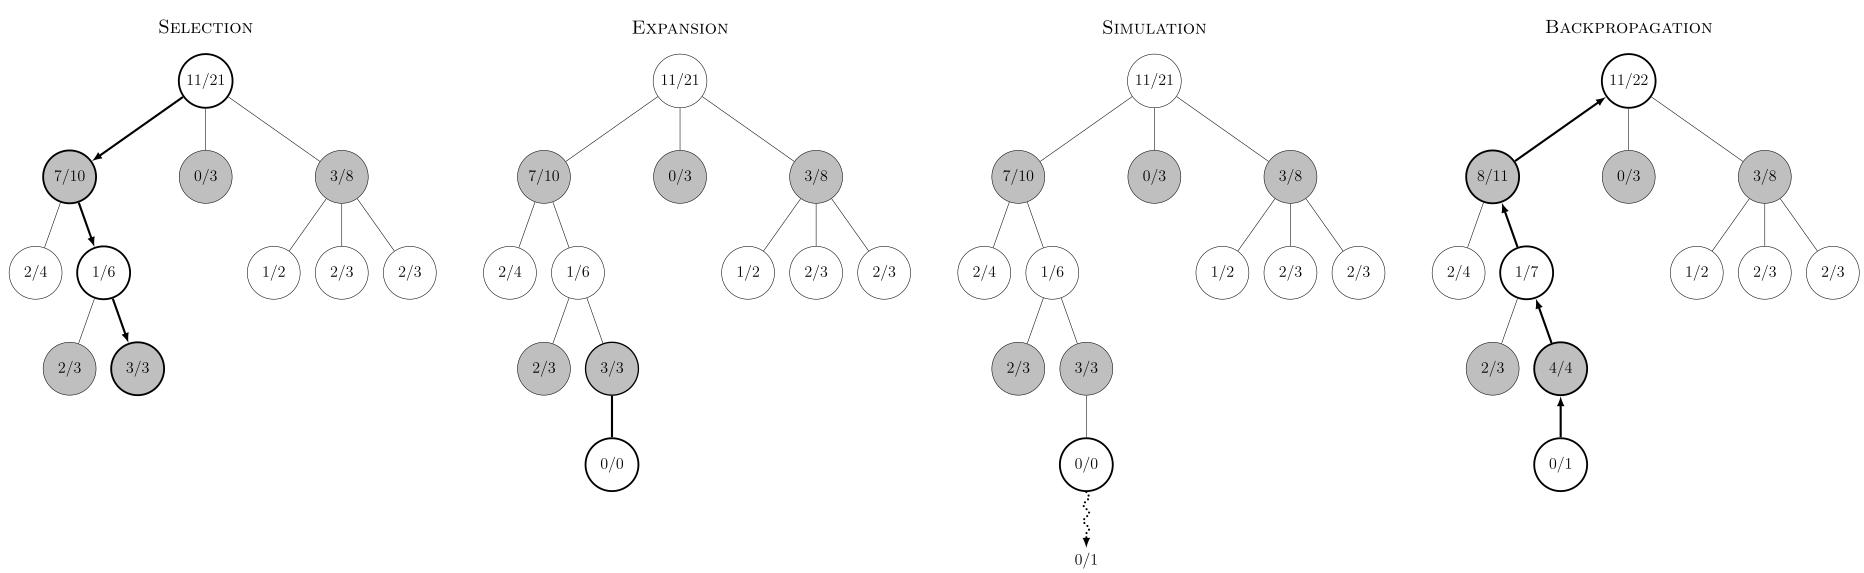
\includegraphics[width=\textwidth]{../assets/MCTS.png}
    \caption{MCTS 算法示意图 \cite{MCTS-steps}}
\end{figure}

当确定了扩展节点之后,算法以该节点为根进行大量的随机模拟,
并根据模拟的结果确定在该根节点下如何落子,并更新祖先节点的估计值,
该策略一般称为默认策略(Default Policy)。在平凡情况下,
算法在每一次模拟中从根节点的状态开始,随机地选择一个落子点 $x$ 进行落子,
接下来不断地交替随机落子直至棋局结束,并根据结束时双方的胜负状态来确定当前状态下
落子点 $x$ 的估计值。当完成大量的模拟之后,对每一种落子点的估计值将变得更为准确,算法以此来决定最终的
落子,并向上依次更新祖先节点的估计值。

事实上,我最后采取了特殊策略,并没有完全按照 ``随机地选择一个落子点 $x$'' 进行落子,
而是

\begin{enumerate}
    \item 如果当前局面下有可以直接获胜的落子点,则直接落子;
    \item 如果对手有可以直接获胜的落子点,则直接落子阻止;
    \item 否则,由于 ``靠中间的落子点更容易导致赢局'',因此按照某一权值分布
            选择落子点,中间的权值更高,边缘的权值更低。
\end{enumerate}

\subsection{UCB1 公式}

上限置信区间(Upper Confidence Bound 1) 公式是解决多臂老虎机问题的一种经典算法,
它的核心思想是在探索和利用之间取得平衡,即在已知的信息中选择最优的行动,
同时也要保证对未知的行动进行探索。UCB1 公式如下:
\begin{equation}
    I(i) = \bar{X}_i + \sqrt{\frac{2\ln n}{T_i(n)}} \label{1}
\end{equation}
其中,$\bar{X}_i$ 是手臂 $i$ 所获得的回报的均值,$n$ 是到当前这一时刻为止所访问的总次
数,$T_i(n)$ 是手臂 $i$ 到目前为止总共所访问的次数。
可以理解为,(\ref{1}) 式中前一部分 $X_i$ 就是对到目前为止已经搜集到的知识的价值,
而后一部分则可以看作是尚未充分探索过的节点需要继续探索的必要性。

\subsection{UCT 算法原理}

我最终结合 MCTS 算法和 UCB1 公式,使用了基于上限置信区间的蒙特卡洛树搜索算法
(Upper Confidence Bound 1 Applied to Tree, UCT) 来解决四子棋问题。
UCT 算法的核心在于使用UCB公式来指导搜索过程,通过计算每个可选步骤的置信上界来决定下一步的行动。
这种方法结合了先深后广的搜索策略,即先对每个步骤进行深度搜索,
然后根据UCB公式的计算结果来扩展搜索范围,从而在有限的计算资源内找到相对较优的解决方案。 

此时 UCT 中 UCB1 算法的公式如下:
\begin{equation}
    I_v(v') = \frac{Q(v')}{N(v')} + c\sqrt{\frac{2\ln N(v)}{N(v')}} \tag{2}
\end{equation}
其中 $v$ 是当前节点,$v'$ 是 $v$ 的子节点,$v \to v'$ 表示的就是一次决策(模拟)。
$Q(\cdot)$ 是回报函数,在四子棋中,我使用\textbf{获胜次数}这一指标,
$N(\cdot)$ 是节点的访问次数。

$c$ 是一个常数,用于平衡探索和利用;理论最优解为 $c = \sqrt{2}$。

\subsection{UCT 算法实现}

以下是 UCT 算法的伪代码:其中 TreePolicy 用于选择节点,Expand 用于扩展节点,
DefaultPolicy 用于模拟,Backup 用于反向传播,BestChild 用于选择最优子节点。

$s(\cdot)$ 表示节点的状态,$f(\cdot)$ 表示状态转移函数,$N(\cdot)$ 表示节点的访问次数,
$Q(\cdot)$ 表示节点的回报。

\subsubsection{UCTSearch}

UCTSearch 函数是 UCT 算法的主函数,用于执行 UCT 算法。

\begin{algorithm}[H]
    \caption{UCT Algorithm - UCTSearch}
    \begin{algorithmic}
        \Function{UCTSearch}{$s_0$}
            \State create root node $v_0$ with state $s_0$
            \While{within computational budget}
                \State $v_l \gets$ TreePolicy($v_0$)
                \State $\Delta \gets$ DefaultPolicy($v_l$)
                \State Backup($v_l$, $\Delta$)
            \EndWhile
            \State \Return BestChild($v_0$, $0$)
        \EndFunction
    \end{algorithmic}
\end{algorithm}

\subsubsection{TreePolicy}

TreePolicy 函数用于选择节点,即根据 UCB1 公式选择最优的子节点。

\begin{algorithm}[H]
    \caption{UCT Algorithm - TreePolicy}
    \begin{algorithmic}
        \Function{TreePolicy}{$v$}
            \While {$v$ is not terminal}
                \If {$v$ has expandable children}
                    \State \Return Expand($v$)
                \Else
                    \State $v \gets$ BestChild($v$, $c$)
                \EndIf
            \EndWhile
            \State \Return $v$
        \EndFunction
    \end{algorithmic}
\end{algorithm}

\subsubsection{Expand}

Expand 函数用于扩展节点,即根据当前节点的状态,选择一个未尝试过的动作,
并创建一个新的子节点。

\begin{algorithm}[H]
    \caption{UCT Algorithm - Expand}
    \begin{algorithmic}
        \Function{Expand}{$v$}
            \State choose a random untried action $a$, the next state is $s'$
            \State $s' \gets f(s(v), a)$
            \State create a new child $v'$ of $v$ with state $s'$
            \State \Return $v'$
        \EndFunction
    \end{algorithmic}
\end{algorithm}

\subsubsection{DefaultPolicy}

DefaultPolicy 函数用于模拟,即根据默认策略模拟一次决策。

\begin{algorithm}[H]
    \caption{UCT Algorithm - DefaultPolicy}
    \begin{algorithmic}
        \Function{DefaultPolicy}{$v$}
            \While{the state of $v$ is not a terminal state}
                \State select a legal action $a$ at random
                \State $s \gets f(s, a)$
            \EndWhile
            \State \Return the reward for state $s$
        \EndFunction
    \end{algorithmic}
\end{algorithm}

\subsubsection{Backup}

Backup 函数用于反向传播,即根据模拟的结果向上依次更新祖先节点的估计值。

\begin{algorithm}[H]
    \caption{UCT Algorithm - Backup}
    \begin{algorithmic}
        \Function{Backup}{$v, \Delta$}
            \While{$v \neq \text{null}$}
                \State $N(v) \gets N(v) + 1$
                \State $Q(v) \gets Q(v) + \Delta(v, p)$
                \State $v \gets \text{ the parent of }v$
            \EndWhile
        \EndFunction
    \end{algorithmic}
\end{algorithm}

\subsubsection{BestChild}

BestChild 函数用于选择最优子节点,即根据 UCB1 公式选择最优的子节点。

\begin{algorithm}[H]
    \caption{UCT Algorithm - BestChild}
    \begin{algorithmic}
        \Function{BestChild}{$v, c$}
            \State \Return $\arg\max_{v' \in \text{ children of }v} \frac{Q(v')}{N(v')} + c \sqrt{\frac{2\ln N(v)}{N(v')}}$
        \EndFunction
    \end{algorithmic}
\end{algorithm}

\subsection{实现细节}

我使用 \texttt{C++} 语言实现了 UCT 算法,具体代码位于 \texttt{src/UCT.cpp} 中。

\section{特殊策略}

除了朴素的 UCT 算法之外,在实际实现中,我通过查找资料 \cite{Connect4-github},发现一些特殊策略可以提高最终结果的准确性。

\subsection{将军/解围策略}

在四子棋中,如果对手有可以直接获胜的落子点,那么我们应该优先选择这个落子点,
以阻止对手获胜。这一策略称为将军/解围策略。

\subsection{中心优势}

在 \cite{Connect4-github} 中提到,中心的落子点更容易导致赢局。类似于围棋,
在四子棋的对弈过程中,由于重力原因,四子棋的棋盘中央即为棋盘底部的中央,
于是我考虑 defaultPolicy 随机走子的基础上,更改底部各子的权重,增大中部的权重,
更容易将棋子下在中部,这样下出妙手的可能性更高,提高了有效模拟的比例。

具体而言,假设棋盘宽度为 $w$,则定义
\begin{equation*}
    \text{weight}(i) = \begin{cases}
        (i + 1)^2, & i \le n/2, \\
        \text{weight}(w - i - 1), & \text{otherwise}.
    \end{cases}
\end{equation*}

在 DefaultPolicy 中,我按照这一权值分布选择落子点。具体而言,先随机
选取 $w_0 \in [0, \sum_i\text{weight}(i)]$ 的值,再根据权值分布选择第一个
\textbf{可行}且满足 $\sum_j\text{weight}(j) \le w_0$ 的 $j$。

\subsection{调整权值}

注意到 UCT 算法中的 $c$ 常数是用于平衡探索和利用的,因此我在实际实现中
也对 $c$ 进行了调整。不同 $c$ 值对最终结果的影响如下表所示:
\begin{table}[H]
    \centering
    \begin{tabular}{||c|c||}
        \hline
        $c$ & 胜率 \\
        \hline
        0.500 & 0.57 \\
        0.600 & 0.6 \\
        0.650 & 0.85 \\
        0.707 & 0.95 \\
        1.000 & 0.6 \\
        \hline
    \end{tabular}
    \caption{不同 $c$ 值对最终结果的影响}
\end{table}
因此我在实际实现中选择了 $c = 0.707$。

\section{统计数据}

最终在 Saiblo 平台上进行的批量测试结果如下图所示:

\begin{figure}[H]
    \centering
    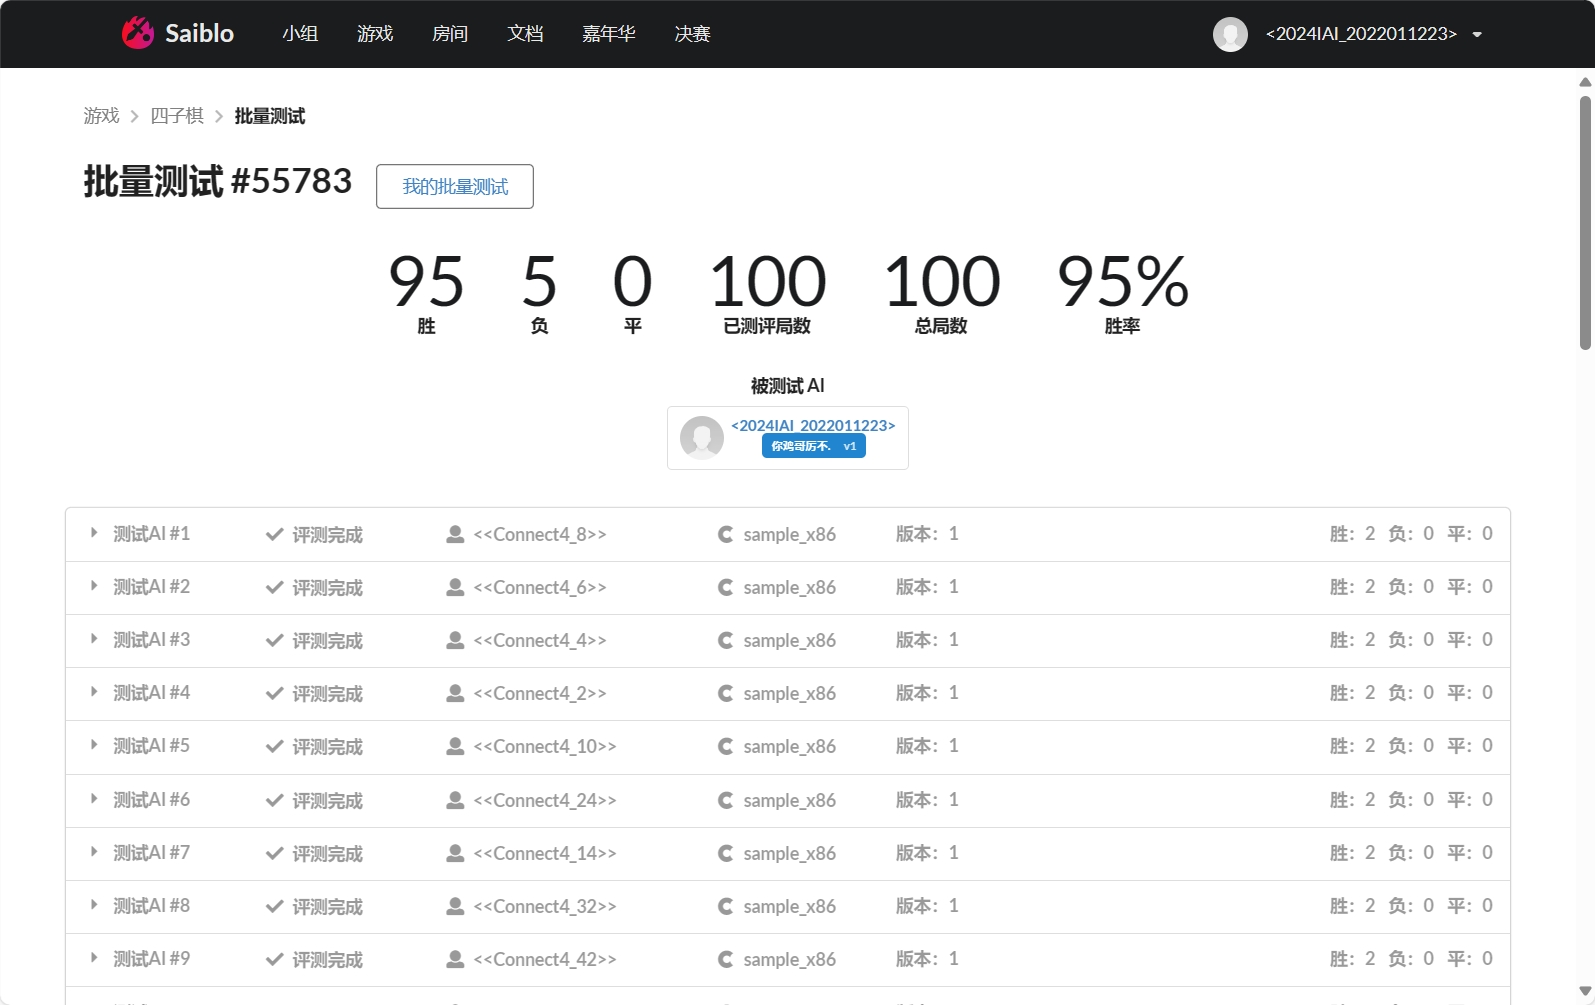
\includegraphics[width=\textwidth]{../assets/result.png}
    \caption{统计数据}
\end{figure}

\section{总结与感想}

通过本次实验,我对蒙特卡洛树搜索算法有了更深入的了解,同时也学会了如何将其应用到
四子棋问题中。在实现过程中,我遇到了很多困难,比如如何设计状态转移函数、如何设计
回报函数、如何设计默认策略等等。通过不断地调试和修改,我最终实现了一个相对较好的
四子棋策略。

在实现过程中,我发现了一些问题,比如在模拟过程中,由于随机性较大,有时候会出现
不合理的落子,导致最终结果不够准确。因此,我在模拟过程中加入了一些特殊策略,
比如将军/解围策略、中心优势等等,以提高最终结果的准确性。

\begin{thebibliography}{99}
    \bibitem{MCTS-steps}
    Robert Moss,
    \emph{File:MCTS-steps.svg - Wikimedia Commons},
    2020,
    \url{https://commons.wikimedia.org/w/index.php?curid=88889583}.
    
    \bibitem{MCTS-wiki}
    \emph{Monte Carlo tree search - Wikipedia},
    2023,
    \url{https://en.wikipedia.org/wiki/Monte_Carlo_tree_search}.
    
    \bibitem{Kocsis2006}
    Levente Kocsis and Csaba Szepesvári,
    \emph{Bandit Based Monte-Carlo Planning},
    In \emph{Machine Learning: ECML 2006},
    Springer, Berlin, Heidelberg, 2006,
    pp. 282--293,
    \url{https://doi.org/10.1007/11871842_29}.
    
    \bibitem{Connect4-github}
    zhaochenyang20,
    \emph{IAI\_2022/homework/connect-4 at main · zhaochenyang20/IAI\_2022 · GitHub},
    2022,
    \url{https://github.com/zhaochenyang20/IAI_2022/tree/main/homework/connect-4}.
\end{thebibliography}

\end{document}
